\noindent\textbf{1.} Gọi số mol khí ban đầu trong mỗi lần lần lượt là $n_A, n_B$ và $n_C$. Sau khi mở van và trạng thái cân bằng được thiết lập, số mol khí là $n_A', n_B', n_C'$. Ở trạng thái cuối, áp suất trong tất cả các phần đều là $p_f$ và nhiệt độ đều là $T_0$. Ta có
\begin{equation*}
  p_{f}V_{A}=n_{A}^{\prime}RT_{0}
\end{equation*}
\begin{equation*}
  p_{f}V_{B}^{\prime}=n_{B}^{\prime}RT_{0}
\end{equation*}
\begin{equation*}
  p_{f}V_{C}^{\prime}=n_{C}^{\prime}RT_{0}
\end{equation*}
kết hợp 3 phương trình trên
\begin{equation*}
  p_{f}(V_{A}^{\prime}+V_{B}^{\prime}+V_{C}^{\prime})=3V_{0}p_{f}=(n_{A}^{\prime}+n_{B}^{\prime}+n_{C}^{\prime})RT_{0}=(n_{A}+n_{B}+n_{C})RT_{0}
\end{equation*}
\begin{equation*}
  \Rightarrow p_{f}=\frac{1}{3V_{0}}(n_{A}+n_{B}+n_{C})RT_{0}=\frac{1}{3V_{0}}(P_{0}V_{0}+P_{0}V_{0}+2P_{0}V_{0})=\frac{4}{3}P_{0}
\end{equation*}
Đối với phần $A$, vì $n_A^{\prime}=n_A$
\begin{equation*}
  p_{f}V_{A}^{\prime}=n_{A}^{\prime}RT_{0}=n_{A}RT_{0}\Rightarrow V_{A}^{\prime}=\frac{3}{4}V_{0}
\end{equation*}
\begin{equation*}
  V_{C}^{\prime}=V_{0}
\end{equation*}
\begin{equation*}
  V_{B}^{\prime}=3V_{0}-V_{0}-\frac{3}{4}V_{0}=\frac{5}{4}V_{0}
\end{equation*}

\noindent\textbf{2.}\\
\noindent\underline{\textbf{Cách 1}}: Vì hệ được duy trì ở nhiệt độ $T_0$, ta có
\begin{equation*}
  \Delta Q_A + \Delta Q_{BC}=0
\end{equation*}
nội năng của phần $A$ là không đổi
\begin{equation*}
  \begin{gathered}
    \Delta Q_{A}=\Delta W=\int_{V_{0}}^{\frac{3}{4}V_{0}}p_{A}dV_{A}=n_{A}RT_{0}\int_{V_{0}}^{\frac{3}{4}V_{0}}\frac{1}{V_{A}}dV_{A}=P_{0}V_{0}\ln\frac{3}{4} \\
    \Rightarrow\Delta Q_{BC}=-\Delta Q_{A}=P_{0}V_{0}\ln\frac{4}{3}\approx0.288P_{0}V_{0}
  \end{gathered}
\end{equation*}

\noindent\underline{\textbf{Cách 2}}: Vì khí được giữ ở nhiệt độ $T_0$, nội năng của nó không đổi
\begin{equation*}
  \Delta Q=\int_{V_{0}}^{\frac{5}{4}V_{0}}p_{B}dV_{B}=\int_{V_{0}}^{\frac{5}{4}V_{0}}p_{A}dV_{B}=\int_{V_{0}}^{\frac{5}{4}V_{0}}\frac{N_{A}kT_{0}}{2V_{0}-V_{B}}dV_{B}=N_{A}kT_{0}\ln\frac{4}{3}=P_{0}V_{0}\ln\frac{4}{3}\approx0.288P_{0}V_{0}
\end{equation*}

\noindent\textbf{3.} Lưu ý rằng, vì quá trình khí di chuyển giữa hai phần $B$ và $C$ là không thuận ngịch, ta không thể sử dụng công thức
\begin{equation*}
  dS=\frac{dQ}{T}
\end{equation*}

\noindent\underline{\textbf{Cách 1}}: Xét một quá trình thuận nghịch có thể đưa hệ từ trạng thái đầu đến trạng thái cuối. Tưởng tượng có một vách ngăn giữa các phần $A+B$ và $C$ có thể di chuyển chậm rãi. Khí trong phần $C$ có thể dãn nỏ do đó áp suất của nó sẽ giảm từ $2P_0$ xuống $P_f$ tại đó thể tích của phần $C$ là $V_1$
\begin{equation*}
  2P_0V_0=\frac{4}{3}P_0V_1\implies V_1=\frac{3}{2}V_0
\end{equation*}
\begin{figure}[h]
  \centering
  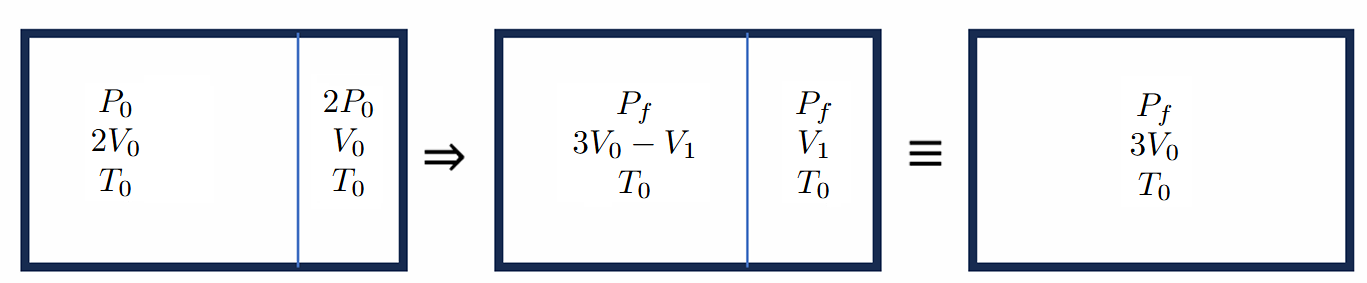
\includegraphics[width=1\textwidth]{Figures/Solutions/Fig 2.1.png}
  \begin{center}
    \figurename{ 2.1}
  \end{center}
\end{figure}

\noindent vách ngăn mà ta tưởng tượng có thể di chuyển từ từ
\begin{equation*}
  \begin{gathered}
    \Delta S=\frac{dQ}{T_{0}}=\frac{pdV}{T_{0}}=\frac{(p_{C}-p_{AB})dV_{C}}{T_{0}} \\
    \Delta S=\int_{V_{0}}^{\frac{S_{0}}{2}V_{0}}\left(\frac{2Nk}{V_{C}}-\frac{2Nk}{3V_{0}-V_{C}}\right)dV_{C}\\
    =2Nk\int_{V_{0}}^{\frac{S_{0}}{2}V_{0}}\left(\frac{1}{V_{C}}-\frac{1}{3V_{0}-V_{C}}\right)dV_{C}=2Nk\left(\ln\frac{3}{2}+\ln\frac{3}{4}\right)=2Nk\ln\frac{9}{8}=2\frac{P_{0}V_{0}}{T_{0}}\ln\frac{9}{8} \\
    \approx0.236\frac{P_{0}V_{0}}{T_{0}}
  \end{gathered}
\end{equation*}

\noindent\underline{\textbf{Cách 2}}: Để tính entropy của phần khí $BC$, ta có thể sử dụng phương trình Sackur-Tetrode cho khí lý tưởng
\begin{equation*}
  \begin{gathered}
    S=Nk\left[\ln\left(\frac{V}{N}\left(\frac{4\pi mU}{3Nh^{2}}\right)^{3/2}\right)+\frac{5}{2}\right]=Nk\left[\ln\left(\frac{V}{N}\left(\frac{2\pi mkT_{0}}{h^{2}}\right)^{3/2}\right)+\frac{5}{2}\right]\\
    =Nk\left(\ln\frac{VT_{0}^{\frac{3}{2}}}{N}+c\right)=-Nk\ln P+C
  \end{gathered}
\end{equation*}
với $T_0$ là hằng số. Entropy ở trạng thái đầu
\begin{equation*}
  S_{i}=-2\frac{P_{0}V_{0}}{T_{0}}\ln P_{0}-\frac{2P_{0}V_{0}}{T_{0}}\ln2P_{0}
\end{equation*}
entropy ở trạng thái cuối
\begin{equation*}
  S_{f}=-4Nk\ln P_{f}=-4Nk\ln\frac{4}{3}P_{0}
\end{equation*}
\begin{equation*}
  \begin{gathered}
    \Delta S=S_{f}-S_{i}\\
    =  -\frac{4P_{0}V_{0}}{T_{0}}\ln\frac{4}{3}P_{0}+2\frac{P_{0}V_{0}}{T_{0}}\ln P_{0}+\frac{2P_{0}V_{0}}{T_{0}}\ln2P_{0}\\
    =\frac{P_{0}V_{0}}{T_{0}}\left(-4\ln\frac{4}{3}P_{0}+2\ln P_{0}+2\ln2P_{0}\right) \\
    \\=\frac{P_{0}V_{0}}{T_{0}}\left(-4\ln\frac{4}{3}+2\ln2\right)=2\frac{P_{0}V_{0}}{T_{0}}\left(\ln\frac{9}{8}\right)\approx0.236\frac{P_{0}V_{0}}{T_{0}}
  \end{gathered}
\end{equation*}